\documentclass[letterpaper,12pt,twoside,]{pinp}

%% Some pieces required from the pandoc template
\providecommand{\tightlist}{%
  \setlength{\itemsep}{0pt}\setlength{\parskip}{0pt}}

% Use the lineno option to display guide line numbers if required.
% Note that the use of elements such as single-column equations
% may affect the guide line number alignment.

\usepackage[T1]{fontenc}
\usepackage[utf8]{inputenc}

% pinp change: the geometry package layout settings need to be set here, not in pinp.cls
\geometry{layoutsize={0.95588\paperwidth,0.98864\paperheight},%
  layouthoffset=0.02206\paperwidth, layoutvoffset=0.00568\paperheight}

\definecolor{pinpblue}{HTML}{185FAF}  % imagecolorpicker on blue for new R logo
\definecolor{pnasbluetext}{RGB}{101,0,0} %


\usepackage{wrapfig,subcaption,array,tabularx,multirow,caption} \usepackage[utf8]{inputenc}

\title{QBUS2820 Assignment2}

\author[]{}


\setcounter{secnumdepth}{0}

% Please give the surname of the lead author for the running footer
\leadauthor{}

% Keywords are not mandatory, but authors are strongly encouraged to provide them. If provided, please include two to five keywords, separated by the pipe symbol, e.g:
 

\begin{abstract}

\end{abstract}

\dates{This version was compiled on \today} 

% initially we use doi so keep for backwards compatibility
% new name is doi_footer

\pinpfootercontents{QBUS2820 Assignment 1}

\begin{document}

% Optional adjustment to line up main text (after abstract) of first page with line numbers, when using both lineno and twocolumn options.
% You should only change this length when you've finalised the article contents.
\verticaladjustment{-2pt}

\maketitle
\thispagestyle{firststyle}
\ifthenelse{\boolean{shortarticle}}{\ifthenelse{\boolean{singlecolumn}}{\abscontentformatted}{\abscontent}}{}

% If your first paragraph (i.e. with the \dropcap) contains a list environment (quote, quotation, theorem, definition, enumerate, itemize...), the line after the list may have some extra indentation. If this is the case, add \parshape=0 to the end of the list environment.


\captionsetup[figure]{labelfont={it,bf,scriptsize},textfont={it,scriptsize},labelsep=colon}
\captionsetup[table]{labelfont={it,bf,scriptsize},textfont={it,scriptsize},labelsep=colon}
\captionsetup[FLOAT_TYPE]{labelformat=simple, labelsep=colon}

\hypertarget{task-a}{%
\section{Task A}\label{task-a}}

\hypertarget{introduction}{%
\section{Introduction}\label{introduction}}

In a traditional manner, sale prices of houses were predicted by
comparing sale prices and costs in the real estate market. There was no
general standard to estimate the value of houses. Machine learning
techniques therefore play an important role to help establishing models
for sale prices of house predictions. As mentioned by Calhoun, the
availability of a house price prediction model helps fill up an
essential information gap and improve the efficiency of the real estate
market (Calhoun, 2003).

This project aims to develop predictive models for sale prices of house
with machine learning techniques. With the sale price which is a
numerical variable being the response of predictive models, six models
are developed and validated.

By comparing the root mean squared errors of predictions, the lasso
regression model and random forest model are found to have the best
predictive performance for the housing data, compared to elastic net,
ridge regression, k-nearest neighbor regression and stepwise regression
with forward selection.

\hypertarget{data-processing-and-exploratory-data-analysis}{%
\section{Data processing and exploratory data
analysis}\label{data-processing-and-exploratory-data-analysis}}

There are 36 numeric variables and 43 categorical variables in the
housing data. By calculating the correlation coefficient, 12 numeric
variables are found to be potentially linearly related to sale price, as
the absolute values of corresponding correlation coefficients are
greater than 0.5. The distributions of these variables are visualized in
figure \ref{fig:scatter}. `TotRms AbvGrd', `Garage Area', `1st Fir SF'
and `SalePrice' are shown to be right-skewed while `Garage Yr Blt' and
`Overall Qual' are left-skewed, but these distributions are
significantly influenced by outliers in several columns. Moreover, some
variables, such as `TotRms AbvGrd', tend to have linear relationships
with other variables except sale price, leading to multi-collinearity.
This could violate the assumption of some predictive models, such as
multiple linear regression, thus robustness to multi-collinearity should
be carefully considered when developing predictive models.

Figure \ref{fig:boxplots} shows the distribution of sale price with
regard to different categorical features. For most categorical features,
sale prices tend to largely different for different groups of the
categorical feature, except `BsmtFin Type 2' and `Land Slope'. However,
although medians sale prices look similar for different groups of
`BsmtFin Type 2' and `Land Slope', the distribution of sale prices are
not identical. Hence, it can still be worthwhile to include these two
variables as features to predict sale price. In addition, the boxplots
also highlight the outliers of sale price existing in different
categorical groups.

Besides affecting the shapes of data distribution, the existing outliers
of numeric variables can also post a significant effect on predictive
performance when making sale price predictions.Therefore data
pre-processing needs to be considered in the stage of feature
engineering in order to overcome issues caused by outliers.

\hypertarget{feature-engineering}{%
\section{Feature engineering}\label{feature-engineering}}

\begin{wrapfigure}{r}{0.5\textwidth}
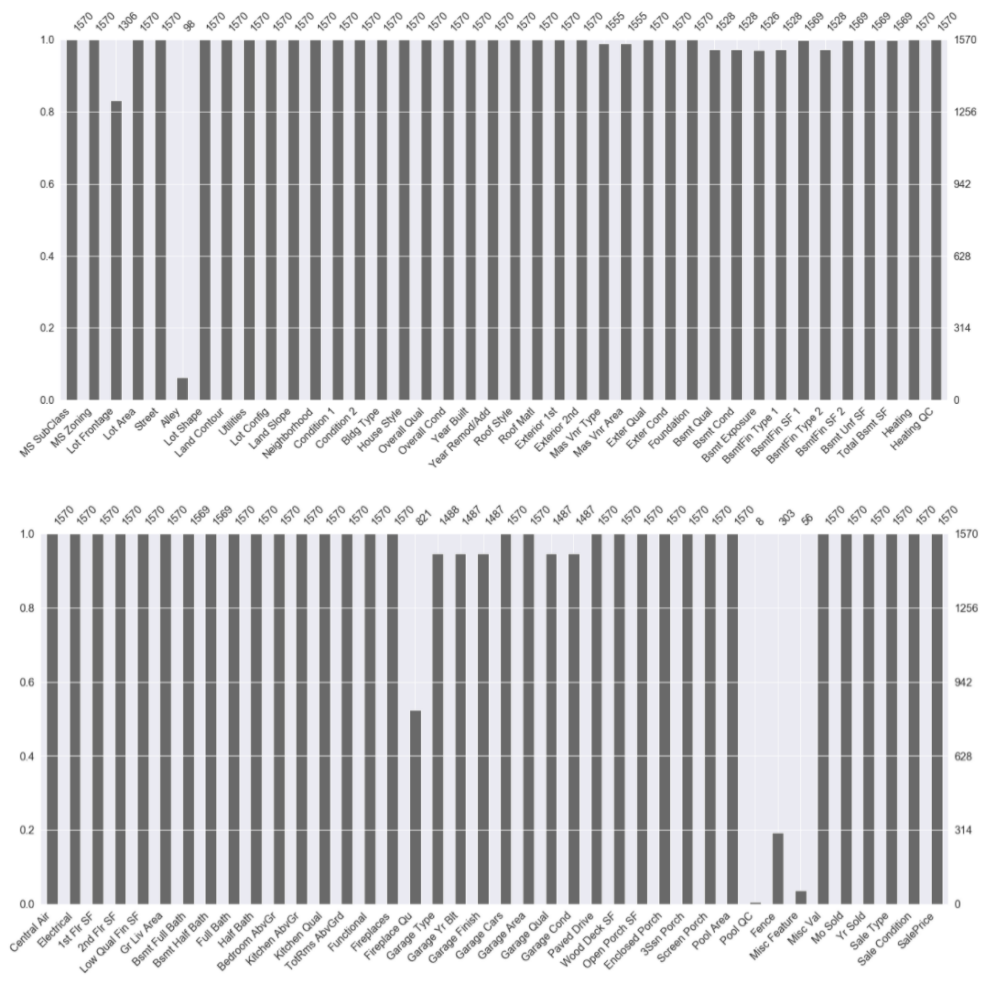
\includegraphics[width=1\linewidth]{miss_plot.png}
\centering
\caption{Visualizing missingness of housing data in training set.}
\label{fig:miss}
\end{wrapfigure}

As shown in Figure \ref{fig:miss}, there are huge amounts of missing
values in several columns: `Alley', `Fireplace Qu', `Pool QC', `Fence',
`Misc Feature', with more than 40\% missing values within each column.
With this issue, such variables are uninformative to be a feature of
predictive models as there are too few observations. To deal with this,
removing all rows with missing values can lead to significant loss of
information, while imputation using small amount of observations can
misrepresent the population for largely incomplete columns. Therefore,
`Alley', `Pool QC', `Fence', `Misc Feature' are abandoned due to high
missing rates.

Besides, there are 19 columns containing missing values but the
percentages of missing values are less than 20\%. This can be deal with
by imputation. The missing values are imputed by using the most frequent
value of each column.

As mentioned before, outliers exist with most of numeric features, which
could be a big concern for predictive performance. Data standardization
is therefore performed for numeric variables by subtracting the mean,
followed by dividing the standard deviation of the corresponding
columns.

After feature engineering, there are 74 informative features, with 36
features being numeric and 38 features being categorical. There are 1570
observations in the training set and 1210 observations in the testing
set. For regression models involving categorical features, dummy
variables are created for each categorical feature.

\hypertarget{methodology}{%
\section{Methodology}\label{methodology}}

Five regression models are trained by two sets of data where one
training set contains numeric features only and the other set includes
both categorical and numeric features. With regards to the issue of
multi-collinearity mentioned before, all of the five regression
techniques used are capable for addressing multi-collinearity. Therefore
there is no need to eliminate features suffering from
multi-collinearity, and all features surviving in the feature
engineering stage are involved in predictive models development.

To develop the best parameter set for each regression models,
hyperparameters are tuned with 5-fold cross validation. The performance
of models with different values of hyperparameters is estimated by
negative mean squared error, where a larger score indicates better
predictive performance. For each machine learning model, the value of
hyperparameter resulting in the best performance is selected to be
optimal.

\hypertarget{random-forest-regression}{%
\subsection{Random forest regression}\label{random-forest-regression}}

A random forest regression model, which is an extension of decision
tree, is developed. It is a supervised learning techniques which applies
ensemble learning method for regression. With this technique, decision
trees are created in parallel by bagging (i.e.~reduce the variance of
predictions by resampling). In this case, the mean predicted sale price
of the individual trees is reported.

As random forest applies bootstrap sampling, multi-collinearity is not a
concern because it is simply selecting different features from training
set to develop models. In addition, the splits of each tree are randomly
sampled from the training set so that with the randomness, overfitting
can be avoided.

The number of features being spitted on at each leaf node which is a
hyperparameter is the main focus to find the optimal random forest
model. Another determinant parameter is the number of trees in random
forest. To tun the random forest model, 10 values of number of trees
(`n\_estimators'), ranging from 200 to 2000, are fed into models. The
maximum number of features being spitted, which is presented as
`max\_feature' in python, is obtained by taking a square root of the
number of feature.

The optimal number of fetures being splitted is 1200 for the training
set with numeric features only. The optimal number changes to 200 when
the model involves both categorical and numeric features.

\hypertarget{lasso-regression}{%
\subsection{Lasso Regression}\label{lasso-regression}}

A lasso regression model is developed as it is able to deal with
multi-collinearity as well as feature selection. As such it is a highly
automate technique with satisfactory predictive performance and
interpretability.

The key component of the lasso model is to perform L1 regularization.
Hence the objective is to minimize
\(\sum^n_{i=1}(y_i-\beta_0-\sum_jx_{ij}\beta_j)^2+\lambda\sum^p_{j=1}|\beta_j|\),
where \(\lambda\) is the hyperparameter which is tuned to control the
strength of L1 regularization penalize. Increasing \(\lambda\) results
in higher level of L1 penalty and thus more features are eliminated.
This also affects the bias-variance tradeoff as a increase of
\(\lambda\) leads to a increase in bias and a decrease in variance.

It might be challenging to initialize a list of lambdas to tun the model
as there is no strict upper boundary of lambdas. Fortunately, the
\texttt{LassoCV} package in python can fit the data and automatically
find out the optimal \(\lambda\) among 100 different values. For the
numeric training set, the optimal value of \(\lambda\) is 921.2 while it
is 130.6 for model including both numeric and categorical features.

\hypertarget{ridge-regression}{%
\subsection{Ridge Regression}\label{ridge-regression}}

A ridge regression which is similar with the lasso regression, is
constructed. In stead of L1 regularization, the ridage regression
applies L2 regularization which does not help selecting features but it
can still overcome the issue of multi-collinearity.

The hyperparameter is \(\lambda\), being similar with that of lasso
regression, to minimize
\(\sum^n_{i=1}(y_i-\beta_0-\sum_jx_{ij}\beta_j)^2+\lambda\sum^p_{j=1}\beta_j^2\).
The \texttt{RidgeCV} package in python helps to fit data and select the
optimal value of lambda from 100 values. The optimal lambdas for numeric
training set and full training set are 113.2 and 9.6 respectively, which
are largely different.

\hypertarget{elastic-nets}{%
\subsection{Elastic Nets}\label{elastic-nets}}

An elastic nets model performs both L1 and L2 regularization, and
integrates the strength of ridge regression and lasso regression. As
such, it is able to perform certain level of feature selection as well
as placing no restriction on the numer of selected variables.

The hyperparameter \(\lambda\) is tuned to minimize
\(\sum^n_{i=1}(y_i-\beta_0-\sum_jx_{ij}\beta_j)^2+\lambda\sum^p_{j=1}(\alpha \beta_j^2+(1-\alpha)|\beta_j|)\).
Being similar to \texttt{RidgeCV} and \texttt{LassoCV}, the
\texttt{ElasticNetCV} package in python selects the optimal value of
\(\lambda\) from 100 different values for the fitted data. The optimal
lambdas are both 65.6 for numeric set and full set.

\hypertarget{stepwise-regression}{%
\subsection{Stepwise regression}\label{stepwise-regression}}

The stepwise regression is simply a multiple linear regression with
feature selection. The farward selection approach starts from a null
model which contains only the constant, and iterate to add different
number of features to the model. For each iteration, all predictors are
add individually to the model to construct \(p-k-1\) models, where \(p\)
is the total number of predictors available, and \(k\) is the number of
predictors involved in models. For a specific value of \(k\), the best
model is selected based on residual sum of square (RSS). Finally, the
optimal stepwise model is selected by comparing the negative root mean
squred error from cross validation, in order to estimate predictive
performance of models involving different number of predictors.

The optimal model with numeric features contains 17 predictors while the
best model including both categorical and numeric variables contains 73
features.

\hspace{1cm}

\begin{wraptable}{r}{8cm}
\begin{tabular}{ |c|c|c| } 
\hline
\textbf{Model / Features} & \textbf{Numeric} & \textbf{Numeric and Categorical} \\
\hline
\textbf{Forward stepwise} & 34470.77 & $5.21\times 10^{15}$ \\ 
\textbf{Lasso} & 34543.61 & 29628.07 \\
\textbf{Ridge} & 34475.68 & 30082.79 \\
\textbf{Elastic net} & 35380.58 & 32844.26 \\
\textbf{Random forest} & 28016.33 & 28805.04\\
\hline
\end{tabular}
\centering
\caption{Summary of predictive performance for regression models. The performance assessement metric is the root mean squared error from cross validation.}
\label{table:cv_errors}
\end{wraptable}

The predictive performance of models developed are validated by root
mean squared error (RMSE) from 5-fold cross validation. Table
\ref{table:cv_errors} summaries the predictive performances of five
regression models for the two training sets. For models including only
numeric features, random forest regressio has the best performance with
the lowest RMSE while other 4 models have similar peroformance. For
models with both numeric and categorical variables, random forest
regression still has the most accurate predictions, followed by lasso
regression.

\hypertarget{validation-set-results-from-kaggle}{%
\section{Validation set results from
kaggle}\label{validation-set-results-from-kaggle}}

\begin{wraptable}{r}{8cm}
\begin{tabular}{ |c|c|c| } 
\hline
\textbf{Model / Features} & \textbf{Numeric} & \textbf{Numeric and Categorical} \\
\hline
\textbf{Forward stepwise} & 40672.34  & 46984.44 \\ 
\textbf{Lasso} & 39910.50 & 29628.07 \\
\textbf{Ridge} & 40141.87 & 38481.91 \\
\textbf{Elastic net} & 38249.77 &  37679.12\\
\textbf{Random forest} & 25405.28 & 28276.96\\
\hline
\end{tabular}
\centering
\caption{Summary of validation set results from kaggle. The performance assessement metric is the root mean squared error from cross validation.}
\label{table:kaggle_results}
\end{wraptable}

Table \ref{table:kaggle_results} summirizes the validation set results
from kaggle, assessing the predictive performance of five regression
models by root mean squared errors. It is inline with table
\ref{table:cv_errors} that random forest and lasso model regression have
the best predictive performance for both training sets. Moreover, random
forest tends to have more accurate predictions for numeric sets compared
to models with both categorical and numeric variables.

\hypertarget{conclusion}{%
\section{Conclusion}\label{conclusion}}

It is noticable from table \ref{table:cv_errors} that the stepwise
regression with forward selection has a poor predictions with a very
large RMSE for training set involving categorical variables, whereas the
predictive performance for numeric set is relatively satisfactory. This
is because when perforaming stepwise regression, the dummy variables
representing categorical variables are treated as numeric variable when
fitting multiple linaer regression.

\hypertarget{references}{%
\section{References}\label{references}}

\begin{itemize}
\tightlist
\item
  Gibson, M., Little, R. and Rubin, D., 1989. Statistical Analysis with
  Missing Data. The Statistician, 38(1), p.82.
\item
  Scikit-learn.org. 2020. 6.4. Imputation Of Missing Values ---
  Scikit-Learn 0.23.2 Documentation. {[}online{]} Available at:
  \url{https://scikit-learn.org/stable/modules/impute.html}.
\item
  Scikit-learn.org. 2020. 6.4. Imputation Of Missing Values ---
  Scikit-Learn 0.23.2 Documentation. {[}online{]} Available at:
  \url{https://scikit-learn.org/stable/modules/impute.html}.
\item
  Hintze, J.L., 1992. Chapter 335: Ridge Regression. In Number cruncher
  statistical system: statistical software. Kaysville, UT: Jerry L.
  Hintze.
\item
  Chakon, O. (2017). Practical Machine Learning: Ridge Regression Vs
  Lasso. Coding Startups: Coders With Entrepreneurial Mindset. Published
  August 3rd, 2017.
\item
  Allison, P. (2012). When Can You Safely Ignore Multicollinearity?
  Statistical Horizons.
\item
  Cross Validated. (2015). What is elastic net regularization, and how
  does it solve the drawbacks of Ridge (L2) and Lasso (L1)? {[}online{]}
  Available at:
  \url{https://stats.stackexchange.com/questions/184029/what-is-elastic-net-regularization-and-how-doesitsolve-the-drawbacks-of-ridge/184031\#184031}.
\end{itemize}

\hypertarget{task-b}{%
\section{Task B}\label{task-b}}

\hypertarget{exploratory-data-analysis}{%
\section{Exploratory data analysis}\label{exploratory-data-analysis}}

\begin{wrapfigure}{r}{0.5\textwidth}
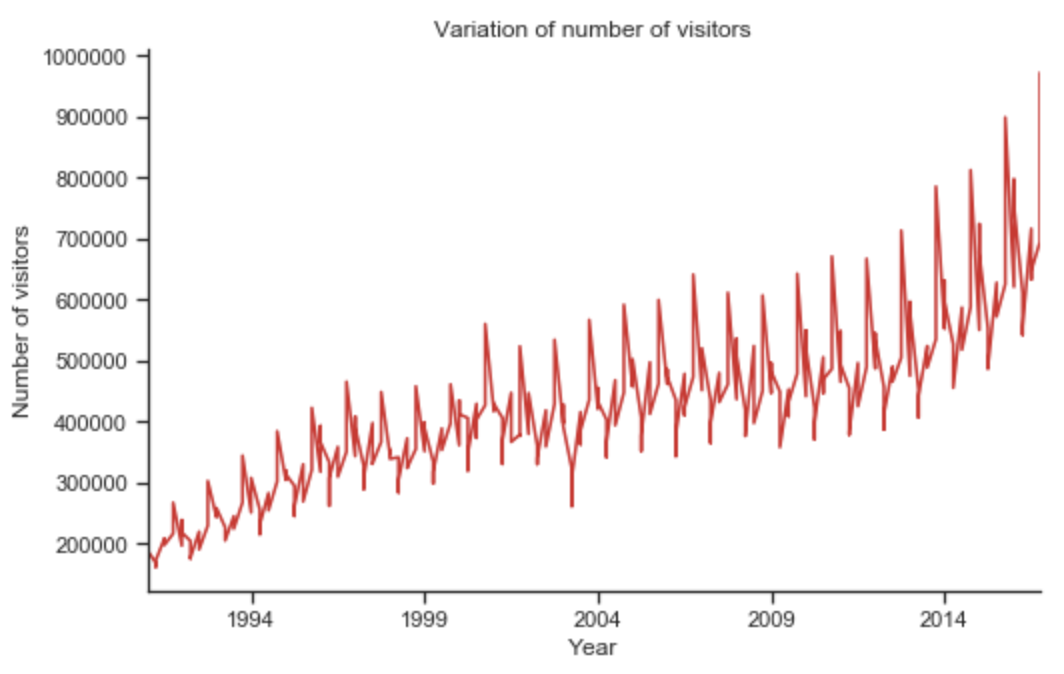
\includegraphics[width=1\linewidth]{timeseries.png}
\centering
\caption{Time series of number of visitors from 1991 to 2016.}
\label{fig:timeseries}
\end{wrapfigure}

The time series plot figure \ref{fig:timeseries} shows an upward trend
from 1991 to 2016, with a seasonal pattern as systematic changes occur
in short periods which are fixed. Furthermore, the variation of number
of visitors within the fixed period becomes greater as time moves. As
such, a multiplicative forecasting model may be more suitable for this
data compared to an additive model.

\hypertarget{forecasting-models}{%
\section{Forecasting models}\label{forecasting-models}}

\hypertarget{seasonal-random-walk}{%
\subsection{Seasonal random walk}\label{seasonal-random-walk}}

\hypertarget{drift-model}{%
\subsection{Drift model}\label{drift-model}}

\hypertarget{exponential-smoothing}{%
\subsection{Exponential smoothing}\label{exponential-smoothing}}

\hypertarget{appendix}{%
\section{Appendix}\label{appendix}}

\begin{figure}
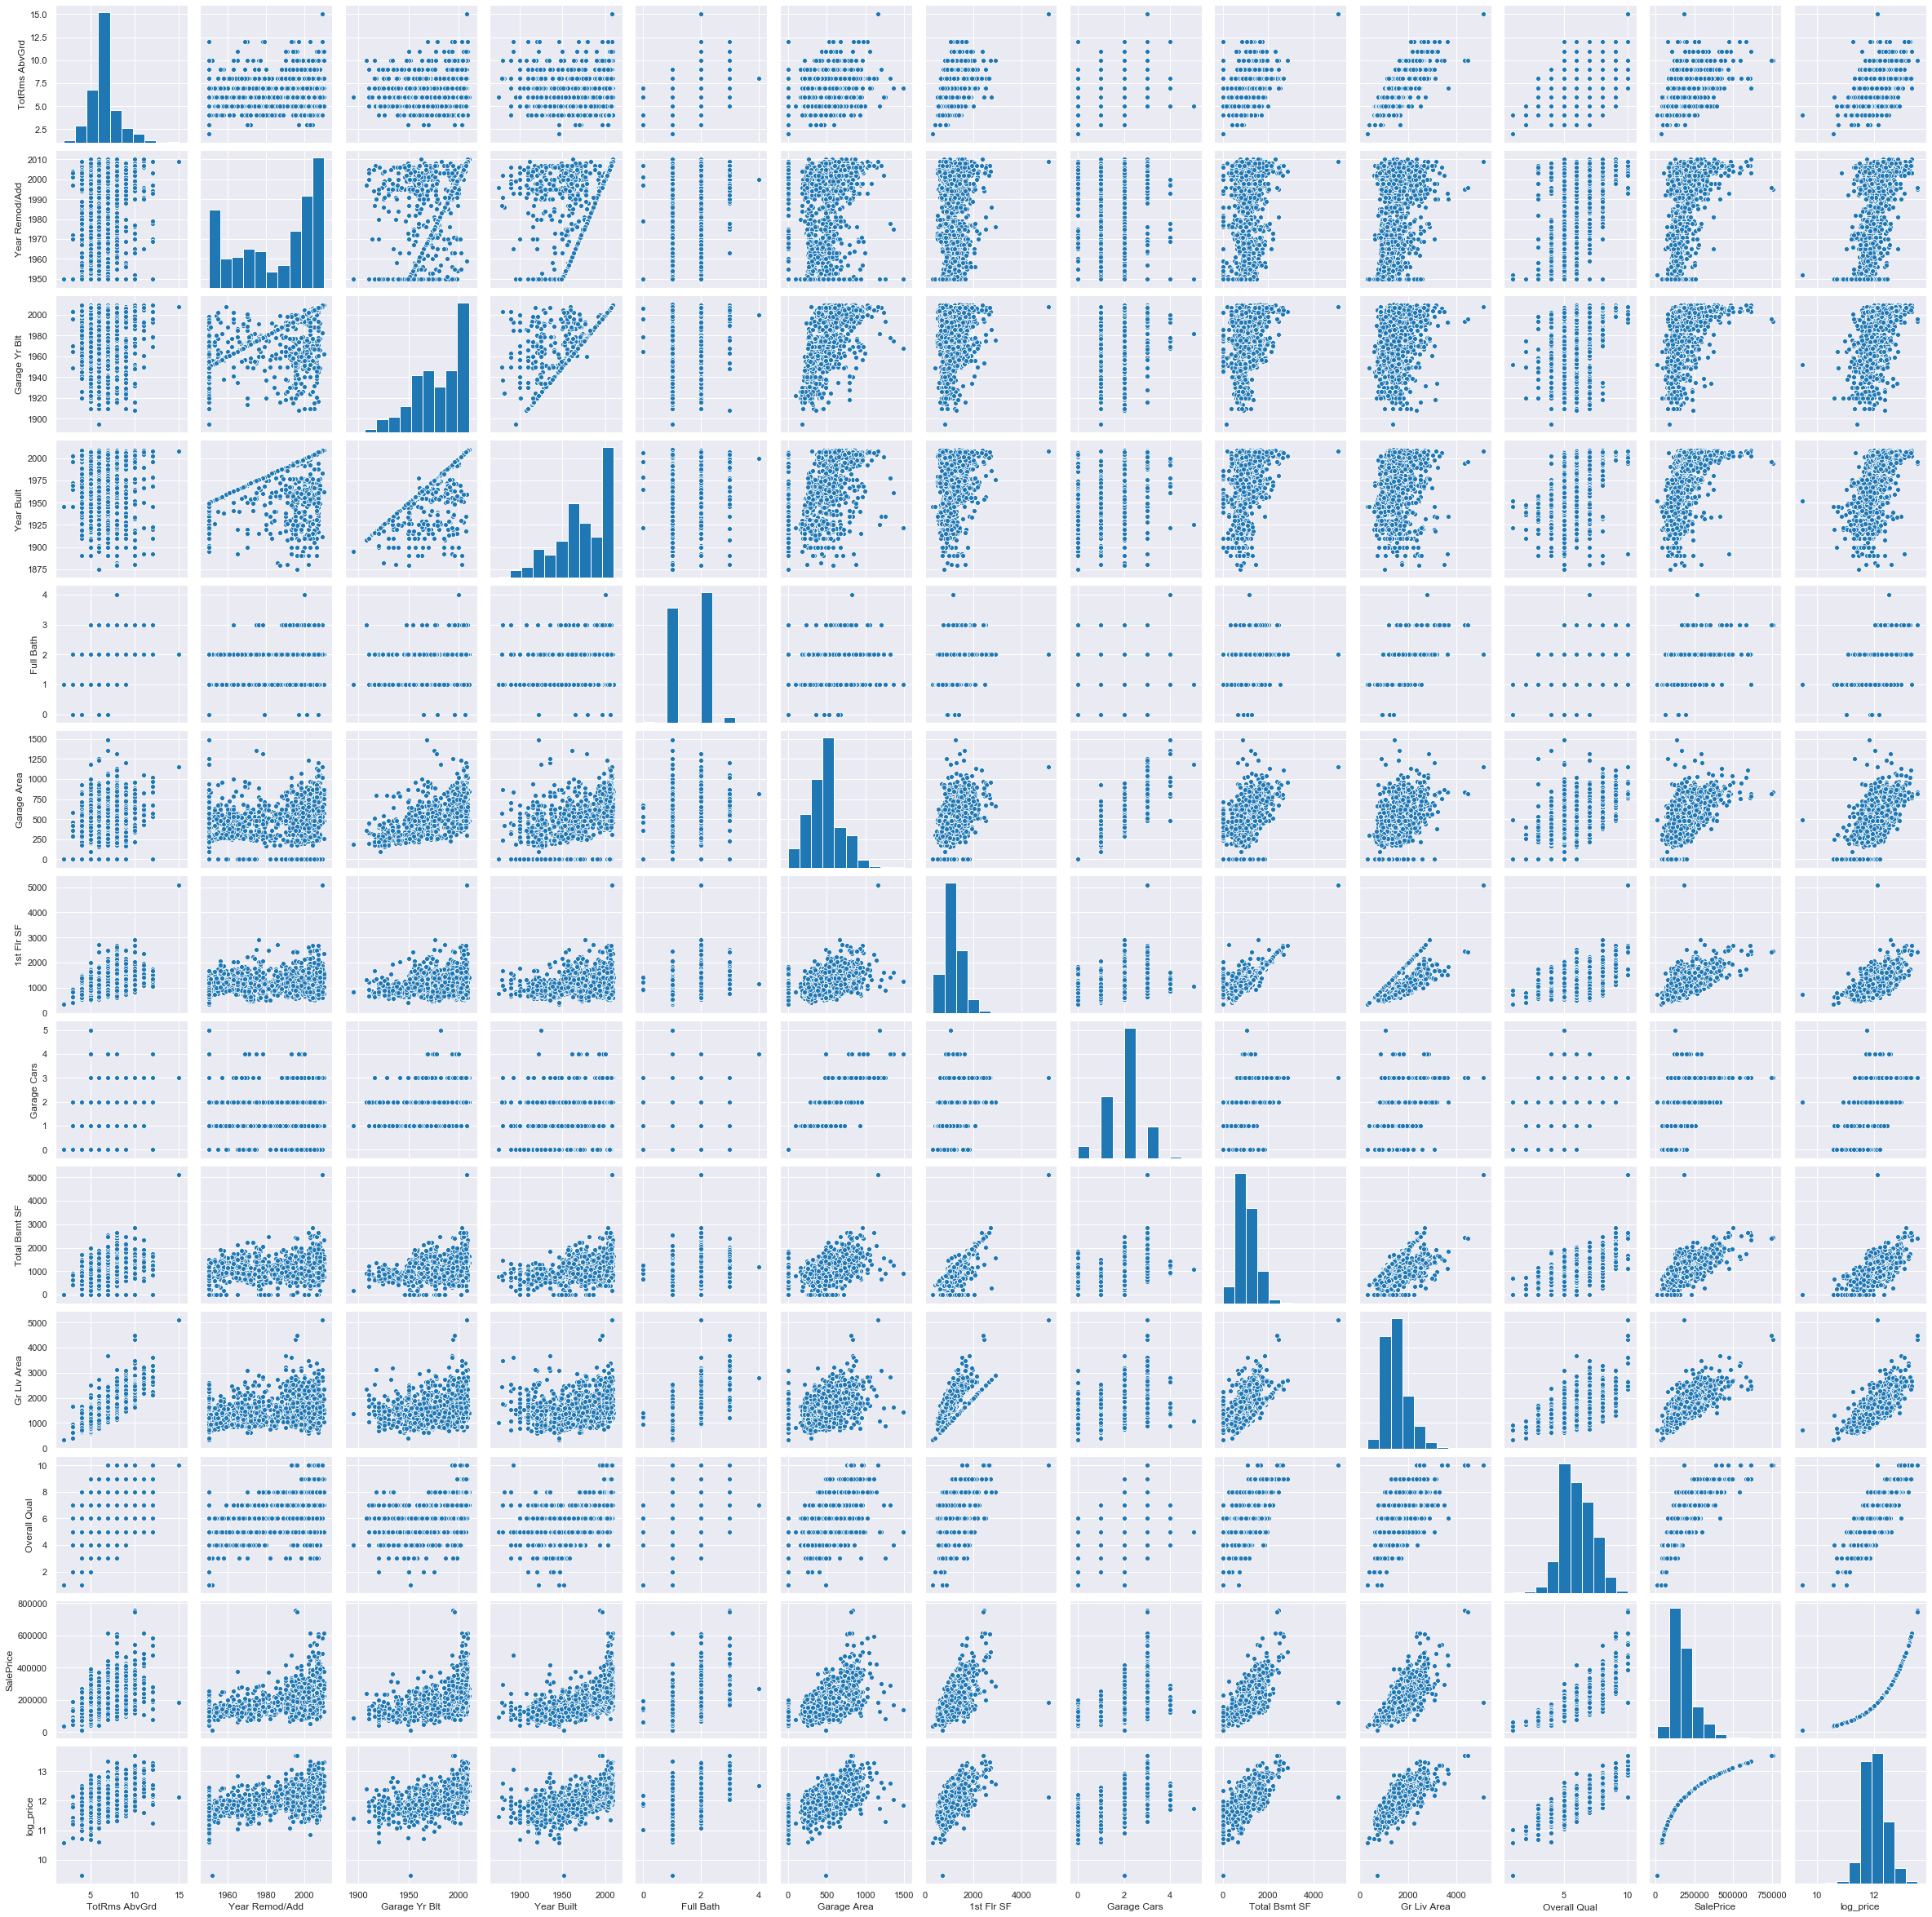
\includegraphics[width=0.8\textwidth]{scatter.png}
\centering
\caption{Distribution of numeric variables in housing data.}
\label{fig:scatter}
\end{figure}

\begin{figure}
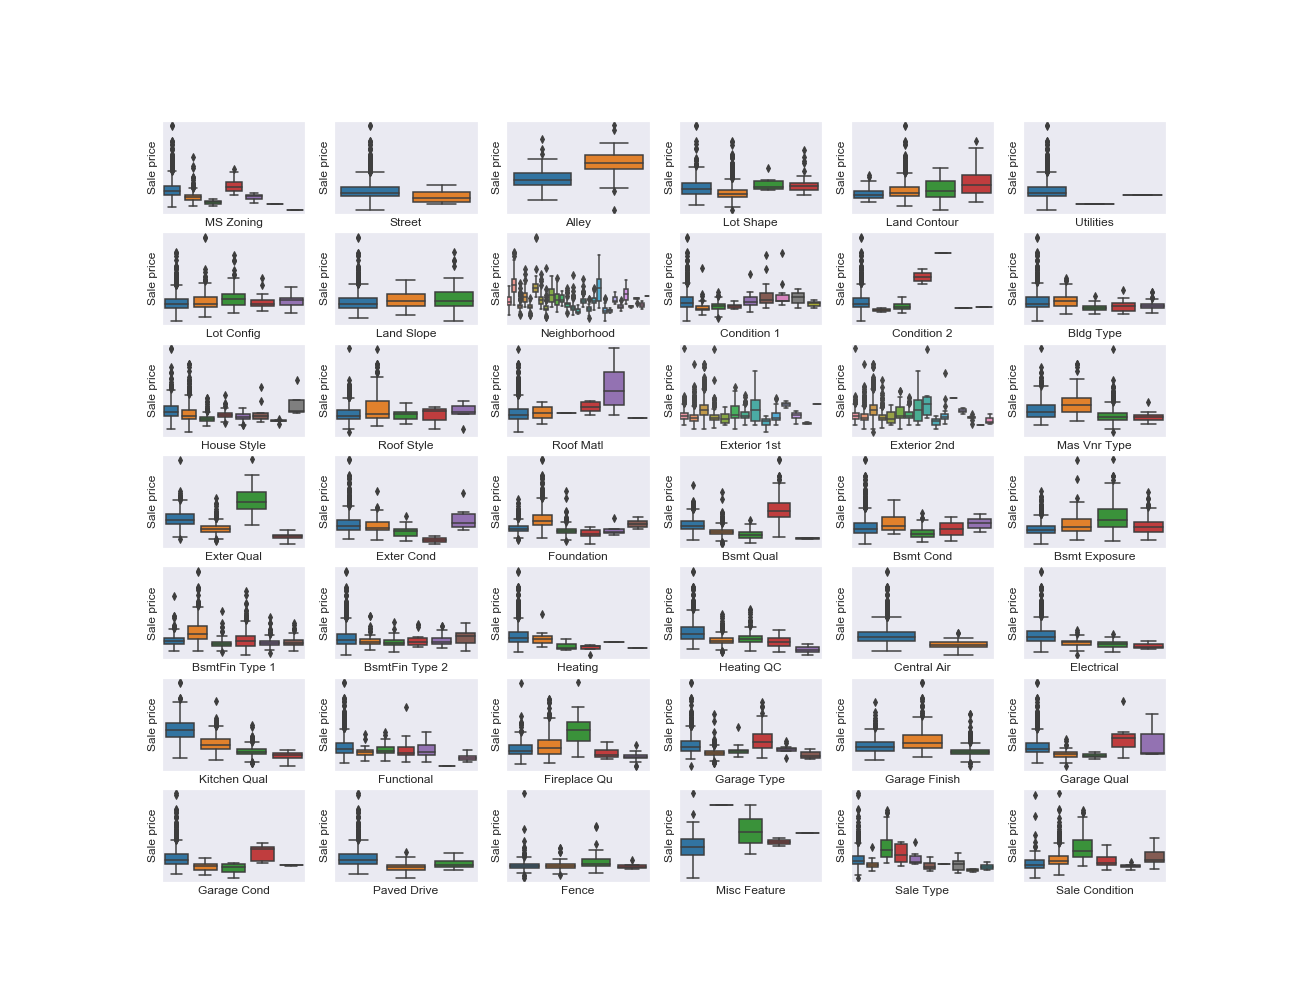
\includegraphics[width=0.8\textwidth]{boxplot.png}
\centering
\caption{Boxplots demonstrating distribution of sale price for houses with different categorical features in housing data.}
\label{fig:boxplots}
\end{figure}

%\showmatmethods


\bibliography{pinp}
\bibliographystyle{jss}



\end{document}

